\documentclass[submit,techreq,noauthor]{eco}	% semi style
\usepackage[dvips]{graphicx}
\usepackage{listings, jlisting} 		% for source code
\usepackage{url}
\usepackage{setspace}
\usepackage{here}
%\setstretch{1.5} % 行間を広くします(資料チェックしてもらうときはコメントを外す)
\lstset{
  basicstyle={\ttfamily},
  identifierstyle={\small},
  commentstyle={\smallitshape},
  keywordstyle={\small\bfseries},
  ndkeywordstyle={\small},
  stringstyle={\small\ttfamily},
  frame={tb},
  breaklines=true,
  columns=[l]{fullflexible},
  numbers=left,
  xrightmargin=0zw,
  xleftmargin=3zw,
  numberstyle={\scriptsize},
  stepnumber=1,
  numbersep=1zw,
  lineskip=-0.5ex
}

\begin{document}

\semino {4/7}					% 年度/回数
\date   {4/11/25/金}				% 平成/月/日/曜日
\title  {Operating System Support for Safe and Efficient Auxiliary Execution}	% タイトル
\author {山下 恭平}				% 氏名

\begin{abstract}
本稿はUSENIX,OSDI'22 に掲載されている論文「Operating System Support
 for Safe and Efficient Auxiliary Execution」\begin{math}^{[1]}\end{math}の内容についてまとめた
ものである.近年のアプリケーションは様々な補助タスクが実行されている.補助タスクとは,アプリ
ケーションが自身のメンテナンス,自己管理を行うタスクのことである.これらのタス
クは、アプリケーションのアドレス空間で実行することで,高い観測性と制御性
を得るが,安全性と性能の問題が発生する.また,補助タスクを別のプロセスで実行す
ると,分離性は高いが,観測性と制御性が劣る.本稿では,この問題を解決するために,
補助タスクに対するサポートとして,orbitと呼ばれるOSの抽象化機能を提案する.

\end{abstract}
\maketitle

\section{はじめに}
運用されているアプリケーションはその実行状況を調査し,最適化し,デバッグし,
制御するために,頻繁にメンテナンスを行う必要がある.かつてはメンテナンスはアプリケ
ーションの管理者が手動で行なっていたが,現在では多くのアプリケーションは,自身
でメンテナンスを行うための補助タスクが行われている.例えばMySQLでは,デッド
ロックを検出するとロールバックを行う機能が存在する.\begin{math}^{[2]}\end{math}
そのため補助タスクはアプリケーションの信頼性や観測性に大きく影響する.
\indent 既存のOSに搭載されているプロセスやスレッドといった抽象化機能は
メインタスクの実行に適した設計がされており,補助タスクの実行には適していない.
そのため,開発者は,分離は強いが観測と制御が非常に限定される(別プロセス)か,
観測と制御は強いが分離はほとんどできない(スレッド)かのどちらかを選ばざる
を得ない.この問題を解決するために,OSの補助タスクに対するサポートを提供する
orbit抽象化を提案する.\\
\indent orbitタスクは,協力な分離を提供する.同時に,状態同期機能により
メインタスクを観測することも可能である.orbitのプロトタイプはLinux kernel 
5.4.91に実装された.orbitの評価を行うためにMySQL,Apacheを含む6つの大規模
アプリケーションから,7つの補助タスクを抽出し,orbitに移行することに成功した.
また,全てのケースでアプリケーションはフォールトから保護されることがわかった.
分離のコストを測定した所.orbitバージョンアプリケーションでは,中央値で3.3
\%のオーバーヘッドが発生した.\\
\indent 本稿では2章でこの研究が行われる背景について述べ,3章でorbitの詳細な
説明を行う,4章でorbitの性能評価を行い,最後の5章では全体のまとめる.

\section{研究の背景}

\begin{figure}[H]
  \centering
  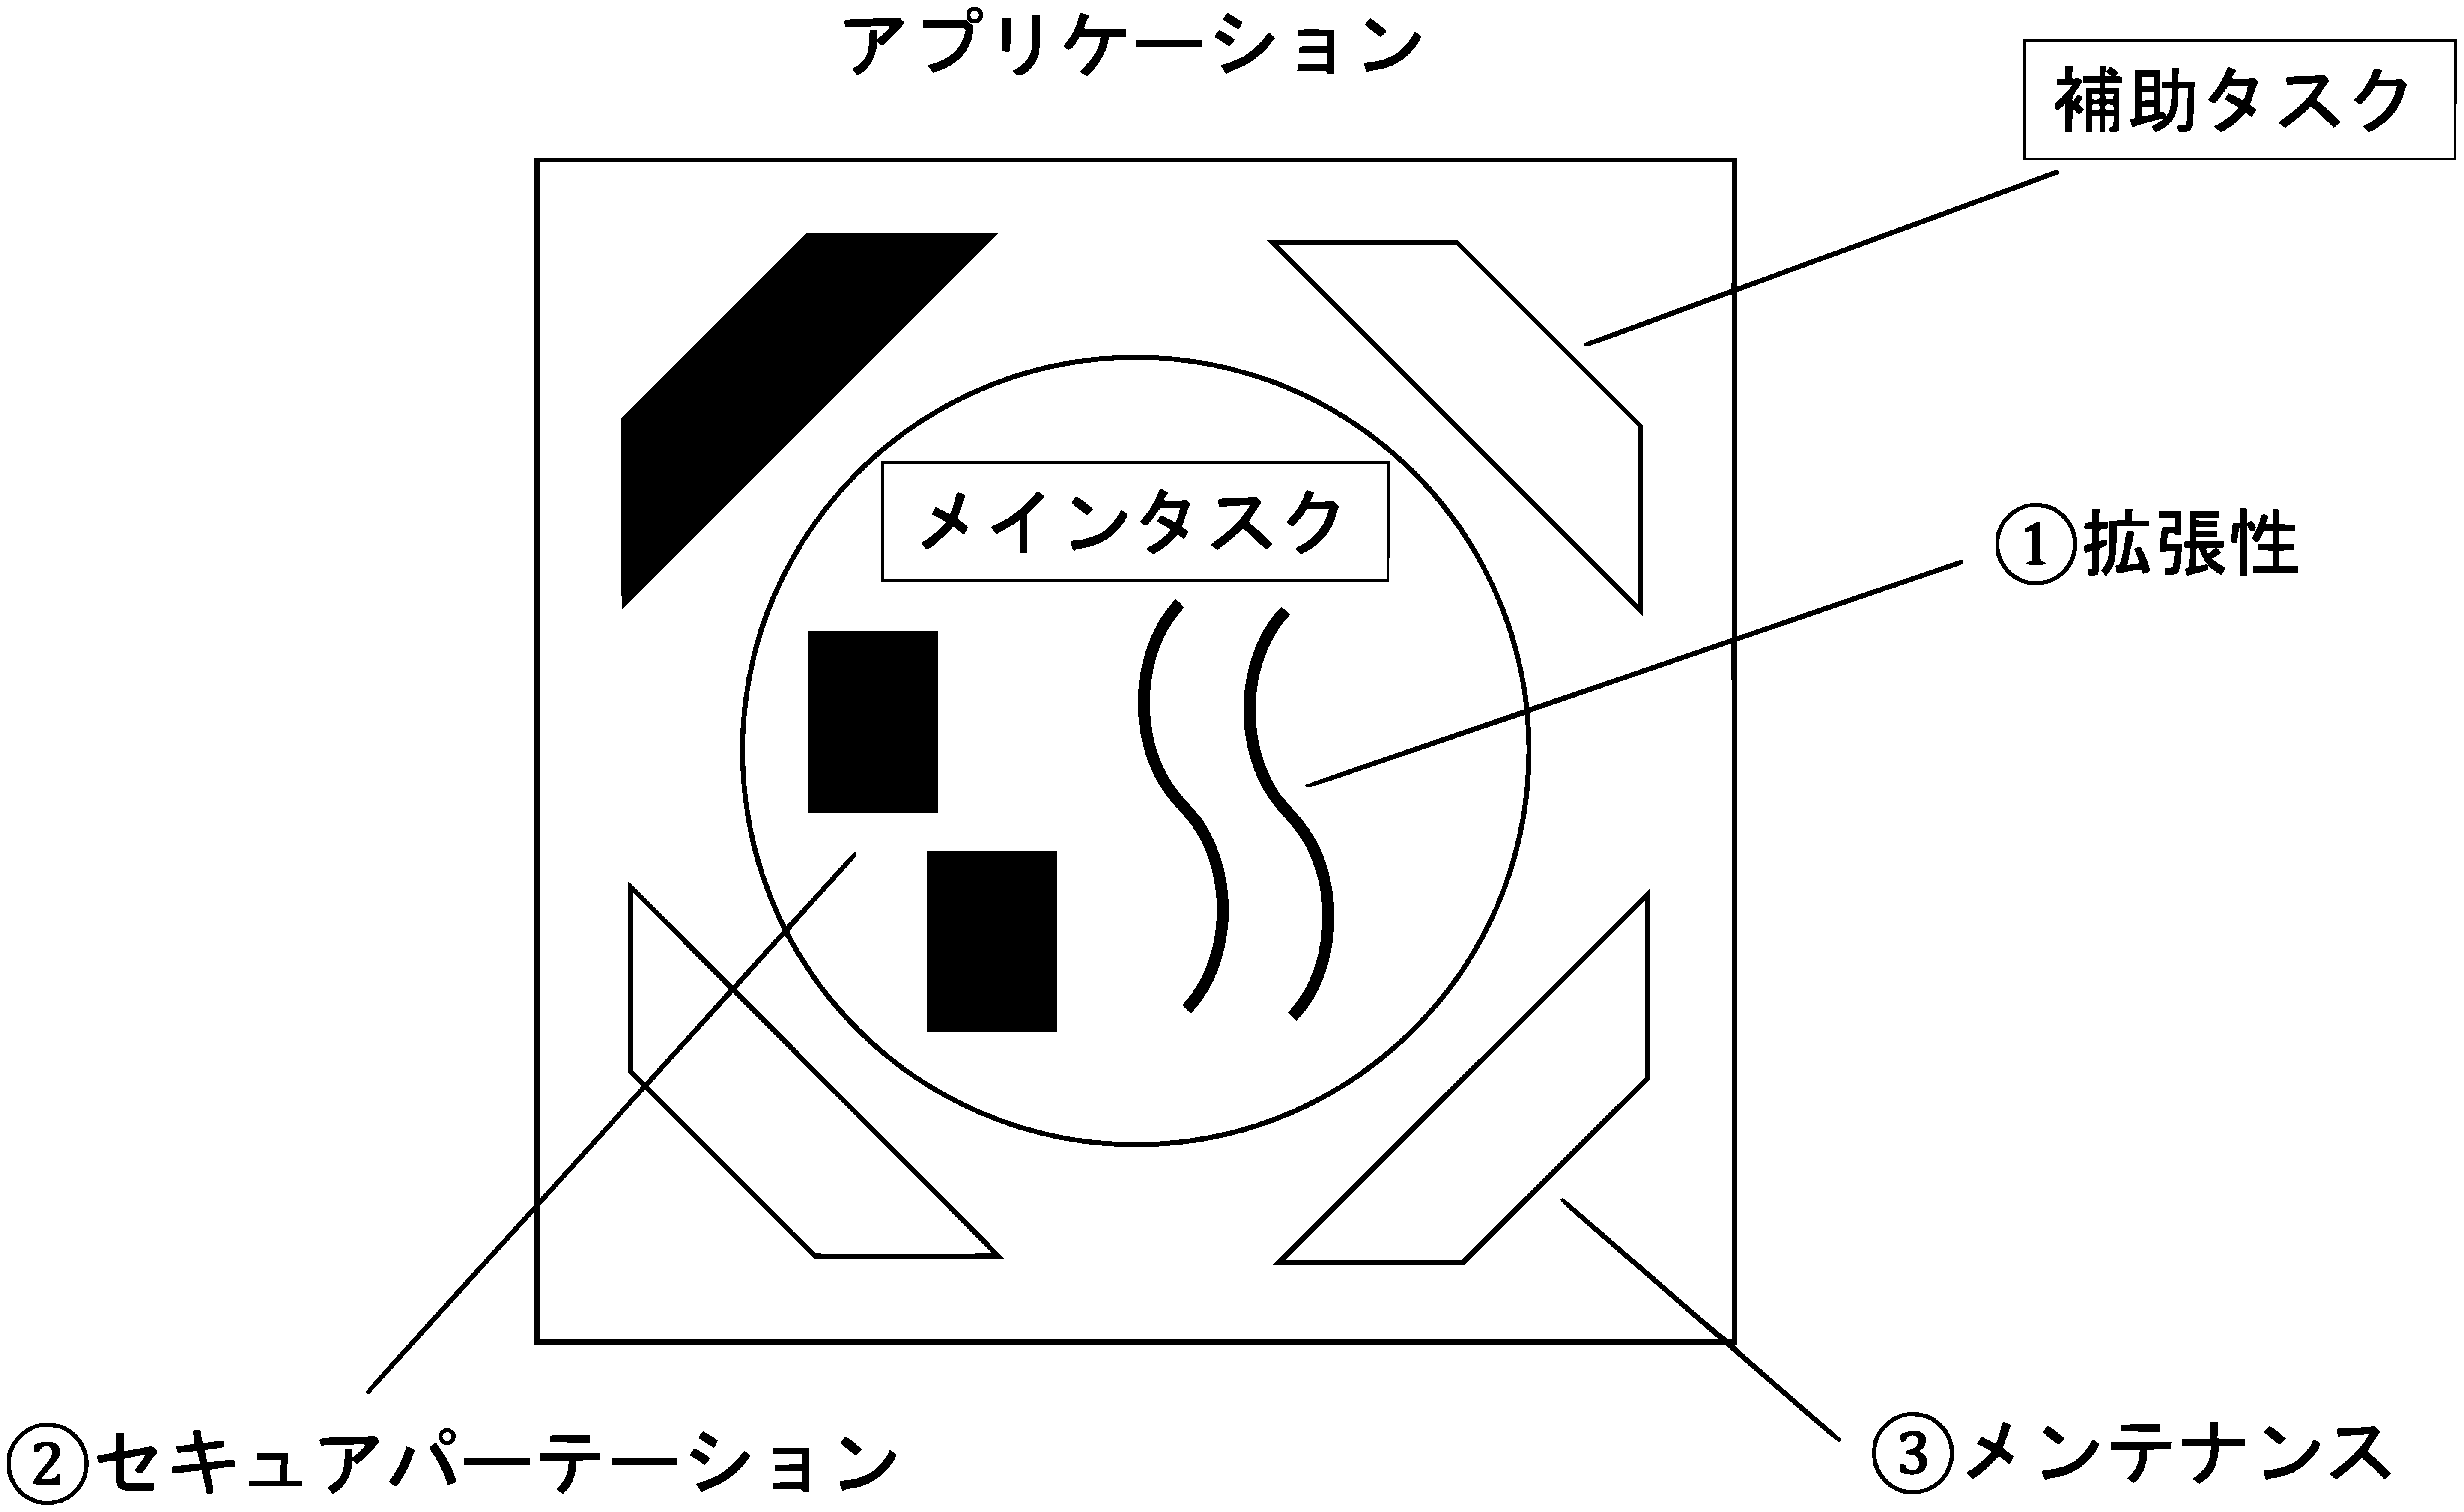
\includegraphics[width=5.5cm]{fig/pic1.eps}
  \caption{アプリケーション構成}
\end{figure}

アプリケーションはメインタスクと補助タスクの2つの論理領域に分けることができる.
図1はアプリケーションの構成を示したものであり,メインタスクの周辺に補助タスクが
存在することがわかる.(1)から(3)については後から説明を行う.補助タスクはメインタスク
のサポートを行うために,、メインタスクを観測し,制御する必要がある.この時,補助タスク
のバグによってがメインタスクに影響が出ないようにするため,メインタスクと補助タスクの
隔離を行う必要がある.つまり,補助タスクには,観測性,制御性,隔離が必要である.

\subsection{タスクの実行方法}
\indent 既存のOSでは補助タスクは主に2種類の実行方法をとる.
1つ目は,メインプログラムと同一のアドレス空間に配置され,メインタスクの関数,
スレッドとして実行される方法だ.この方法であれば,補助タスクはメインタスクの観測,制御が
容易に行うことができる.しかし,補助タスクによってメインタスクが不必要なブロックが起こる
可能性や,補助タスクにバグが存在した場合,メインタスクにまで影響が出るため,隔離について不十分
である.
2つ目はメインタスクと補助タスクを別プロセスで実行する方法だ.この方法であれば,
メインタスクと補助タスクは異なるアドレス空間に存在するため,隔離が十分に行えている.しかし,
メインタスクの観測と制御が困難になる.プロセスやスレッドといった機能は1章で述べた通り,
補助タスクの実行には適していないことがわかった.

\subsection{タスク実行の保護}
\indent タスク実行を保護するOSのサポートは既に多く研究,提案されている.しかし,それらは
異なる2つの目的のために設計されている.\\
1つはアプリケーションの拡張性のためである(図1,(1)).
具体的にはSFI\begin{math}^{[3]}\end{math}という技術がある.SFIとは,アプリケーションバイナリ
を書き換えることで,アプリケーション内の信頼できないコードのメモリアクセスを制限する
ソフトウェア隔離技術ことである.この技術はブラウザの拡張機能などの第三者が作成した
プログラムをアプリケーション内で動作させるときに有効である.\\
2つ目は,セキュアなパーテーショニングを提供するものだ(図1,(2)).具体的には
Wedge\begin{math}^{[4]}\end{math}やlwC\begin{math}^{[5]}\end{math}
といったものがある.これにより,アプリケーションが侵害された場合に,メインタスクの
機密な手続きを守ることができる.\\
しかし,これらの仕組みはアプリケーションのメンテナンス(図1,(3))にとっては不十分である.
その理由として,まず,補助タスクはアプリケーションの開発者と同一人物,機関によって開発さ
れているため,信頼できるものである.また,補助タスクはメインタスクと対話的であり,メインタス
クの状態を常に監視し,場合によっては変更を加える必要があるからだ.次の章では補助タスクの
サポートに求められるものについて述べる.

\subsection{補助タスクの安全性と性能}
1章で述べたように,メインタスクと補助タスクが同一のメモリ空間に存在する場合,補助タスクのバグに
より,無効なメモリにアクセスをした場合アプリケーション全体がクラッシュすることが考えられる.
メインタスクと補助タスクを分離した場合,補助タスクのバグによってアプリケーション全体が
クラッシュする事態は防ぐことができる.しかし,分離された補助タスクによってメインタスクの
性能が大きく低下する場合がある.MySQLのデッドロック検出タスクを実行した状態で,性能
を測定したところ,スループットが最大で79.5\%低下することが報告されている.\begin{math}^{[6]}\end{math}
このことから,補助タスクはアプリケーションの性能を維持,向上させる機能を持っているのにも関わらず,
逆にアプリケーションに害を与える可能性が存在する.\\
\indent 補助タスクの安全性と性能に関する懸念に対処するために,Fork-based Execution Model とSandbox-based Execution Modelという2つの
代替案がある.

\subsubsection*{Fork-based Execution Model}

\subsubsection*{Sandbox-based Execution Model}


\section{orbitについて}


\section{orbitの性能評価}


\section{おわりに}



% 参考文献はここに記述
\begin{thebibliography}{99}
  \bibitem{orbit} Yuzhuo Jing , Peng Huang . Operating System 
  Support for Safe and Efficient Auxiliary Execution , 16th 
  USENIX Symposium on Operating Systems Design and Implementation ,
   page 633 - 648 (2022).
  \bibitem{MySQL} Oracle. MySQL's deadlock detection.\\
  \url{https://dev.mysql.com/doc/refman/8.0/en/innodb-deadlock-detection.html}
  (11/25/2022)
  \bibitem{SFI} R. Wahbe, S. Lucco, T. E. Anderson, and S. L. Graham .
  : Efficient software-based fault isolation. In Proceedings of the 
  Fourteenth ACM Symposium on Operating Systems Principles, SOSP '93,
   page 203 - 216 , (1993).
  \bibitem{Wedge}A. Bittau, P. Marchenko, M. Handley, and B. Karp. 
  Wedge: Splitting applications into reduced-privilege compartments.
   In Proceedings of the 5th USENIX Symposium on Networked Systems 
   Design and Implementation, NSDI '08, page 309 - 322, (2008).
  \bibitem{lwC}J. Litton, A. Vahldiek-Oberwagner, E. Elnikety, D. 
  Garg, B. Bhattacharjee, and P. Druschel. Light-weight contexts: 
  An OS abstraction for safety and performance. In Proceedings of
  the 12th USENIX Conference on Operating Systems Design and Implementation,
   OSDI '16, page 49-64, (2016).
  \bibitem{MySQL}InnoDB deadlock detection is CPU intensive with many locks on a single row.
    \url{https://bugs.mysql.com/bug.php?id=49047} . (11/25/2022)
\end{thebibliography}

\end{document}
